\chapter{Methodik und Umsetzung des Plugins}
\label{chap:umsetzung}

\section{Konzeption}

Zu Beginn der Arbeit existierten nur wenige Anforderungen für das in \autoref{chap:einleitung} definierte Ziel, welche der Ausschreibung des Themas dieser Arbeit entstammen und in einem \textit{Abstract} \citep{ausschreibung} verfasst wurden. Nach gemeinsamer Diskussion und Einarbeitung ergaben sich dadurch die im Folgenden beschriebenen Anforderungen.

\begin{table}[H]
\begin{tabularx}{\textwidth} { 
  | X | X | }
 \hline
 Anforderung & \textit{Dashboard} \\
 \hline
Beschreibung  & Das zu entwickelnde \textit{Plugin} soll ein \textit{Dashboard} zur Verfügung stellen, über das die wichtigsten Eigenschaften eines \textit{Pull Requests} visualisiert werden. \\
\hline
\end{tabularx}
\caption{1. Anforderung: \textit{Dashboard}}
\end{table}

\begin{table}[H]
\begin{tabularx}{\textwidth} { 
  | X | X | }
 \hline
 Anforderung & \textit{Portlets} für das \textit{Dashboard} \\
 \hline
Beschreibung  & Die in dem \textit{Dashboard} angezeigten Eigenschaften eines \textit{Pull Requests} sollen durch andere \textit{Plugins} bereitgestellt werden. \\
\hline
\end{tabularx}
\caption{2. Anforderung: \textit{Portlets}}
\label{tab:portlets}
\end{table}

\begin{table}[H]
\begin{tabularx}{\textwidth} { 
  | X | X | }
 \hline
 Anforderung & Konfiguration \\
 \hline
Beschreibung  & Das \textit{Dashboard} soll konfigurierbar sein, d.\,h. der Nutzer kann bestimmen, wie das \textit{Dashboard} aufgebaut ist und welche \textit{Portlets} in welcher Form angezeigt werden. \\
\hline
\end{tabularx}
\caption{3. Anforderung: Konfiguration}
\end{table}

\begin{table}[H]
\begin{tabularx}{\textwidth} { 
  | X | X | }
 \hline
 Anforderung & \ac{api} für andere \textit{Plugins} \\
 \hline
Beschreibung  & Damit andere \textit{Plugins} solche \textit{Portlets} aus \autoref{tab:portlets} bereitstellen können, muss eine \ac{api} konzeptioniert und entwickelt werden. \\
\hline
\end{tabularx}
\caption{4. Anforderung: \ac{api}}
\end{table}

\begin{table}[H]
\begin{tabularx}{\textwidth} { 
  | X | X | }
 \hline
 Anforderung & Distribution \\
 \hline
Beschreibung  & Das zu entwickelnde \textit{Plugin} soll unter der \textit{MIT}-Lizenz als \textit{Jenkins} \textit{Plugin} veröffentlicht werden, sodass dieses über das \textit{Jenkins Update Center} zu finden ist \citep{jenkinsci_plugin_center}. \\ \hline
\end{tabularx}
\caption{5. Anforderung: Distribution}
\end{table}

Die Art und Weise der Umsetzung der einzelnen Anforderungen entschied sich größtenteils erst während der Einarbeitung bzw. der Arbeit selbst, beispielsweise durch das Feedback anderer Entwickler. Da ein neues \textit{Plugin} erschaffen werden sollte, bestanden auch keine Abhängigkeiten zu anderen \textit{Plugins}. Optional wurde als Ziel festgehalten, die ersten \textit{Portlets} in anderen \textit{Plugins} zu implementieren, sodass das \textit{Plugin} im besten Fall im Rahmen dieser Arbeit bereits durch andere Nutzer verwendet werden kann. Zunächst soll in \autoref{chap:realisierung} die technische Realisierung dokumentiert werden, bevor in \autoref{chap:ergebnisse} die Ergebnisse präsentiert werden.

\section{Realisierung}
\label{chap:realisierung}
Im Rahmen der vorliegenden Arbeit wurde ein \textit{Jenkins Plugin} entwickelt. Es wird dessen Entwicklung und die verschiedenen Komponenten erläutert, die zur Umsetzung der in \autoref{chap:umsetzung} definierten Anforderungen maßgebend sind. Zur Veranschaulichung des Zusammenspiels der einzelnen Klassen soll \autoref{fig:uml} dienen. Es zeigt ein vereinfachtes UML-Klassendiagramm der für die zu implementierenden \textit{Plugins} bedeutsamen Klassen. Im Folgenden werden diese erläutert und ihre Funktion beschrieben werden. Aus Gründen der Übersichtlichkeit wird die Code-Dokumentation in den ausgewiesenen Code-Beispielen entfernt. Die jeweilige Originalquelle wird referenziert.

\begin{figure}[H]
\centering
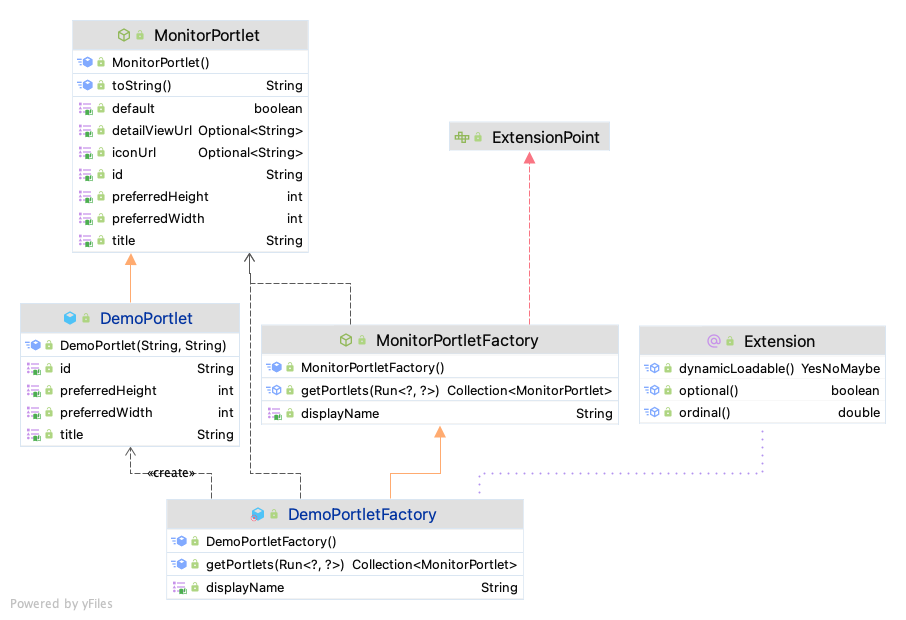
\includegraphics[width=\textwidth]{source/images/uml-with-methods}
\caption[Vereinfachtes UML-Klassendiagramm der für die zu implementierenden \textit{Plugins} relevanten Klassen.]{Vereinfachtes UML-Klassendiagramm der für die zu implementierenden \textit{Plugins} relevanten Klassen, Quelle: Eigene Darstellung.}
\label{fig:uml}
\end{figure}

\subsection{Abstrakte Klassen}
\label{chap:abstractClass}
Die in dem \textit{Plugin} vorhandenen abstrakten Klassen fungieren als Schnittstelle für \textit{Plugins}, die ein \textit{Portlet} bereitstellen möchten. Die beiden abstrakten Klassen \textit{MonitorPortletFactory} und \textit{MonitorPortlet} werden dabei stets zusammen verwendet und stehen in einer \textit{1}:\textit{n}-Beziehung. Jedes \textit{Plugin} besitzt eine \textit{MonitorPortletFactory}, die die \textit{MonitorPortlets} erzeugt und ausliefert. Diese \textit{<<create>>} Beziehung ist in \autoref{fig:uml} veranschaulicht. 
Dadurch wird sichergestellt, dass ein \textit{Plugin} gegebenenfalls mehrere Instanzen der Klasse \textit{MonitorPortlet} bereitstellen kann. Dieser Aspekt ist für die Entwicklung des \textit{Portlets} für das \textit{Warnings Next Generation Plugin} von Bedeutung, welches in \autoref{chap:warnings-ng} vorgestellt wird. Damit das implementierende \textit{Plugin} die beiden Klassen verwenden kann, bedarf es einer Referenz des \textit{Pull Request Monitoring Plugins} in der \textit{pom.xml}, dem \textit{Project Object Model}. Darin werden alle wichtigen Aspekte des Projektes, wie Projektinformationen oder  Projektbeziehungen, also Abhängigkeiten zu anderen Projekten beschrieben. Diese zentrale Steuerungsdatei wird verwendet, um mithilfe des auf \textit{Java} basierenden Build-Managment-Tools \textit{Maven} das Projekt zu verwalten und zu steuern \citep{horn_maven}. Alle \textit{Jenkins} \textit{Plugins} sind in \textit{Java} geschrieben und nutzen dieses Build-Managment-Tool \citep{jenkinsci_plugin}.

\lstinputlisting[escapeinside={(*@}{@*)},caption=Auszug der Datei \textit{plugin/pom.xml} aus dem \textit{Warnings Next Generation Plugin} \citep{warnings-ng-plugin}.,label=listing:pom]{source/listings/pom.xml}

\autoref{listing:pom} demonstriert die Referenzierung anhand des \textit{Warnings Next Generation Plugins}. Zeile \autoref{listing:pom22} deklariert die Abhängigkeit als optional. Dadurch wird diese Abhängigkeit nur dann verwendet, wenn die zugehörige Funktionalität tatsächlich benutzt wird. Wird diese Funktionalität nicht benutzt, so wird auch die Abhängigkeit nicht verwendet.

\subsubsection{\textit{MonitorPortlet}}
Die \textit{MonitorPortlet} Klasse definiert die für ein \textit{Portlet} zu implementierenden Methoden. Ein \textit{Plugin}, welches ein oder mehrere \textit{Portlets} bereitstellen möchte, muss von dieser abstrakten Klasse erben und die Methoden implementieren und gegebenenfalls überschreiben, falls die vordefinierte Implementierung nicht dem jeweiligen Zweck entspricht. \autoref{listing:MonitorPortlet} zeigt die abstrakte Klasse mit ihren Methoden. Ein Titel (vgl. Zeile \autoref{listing:MonitorPortlet3}), eine eindeutige ID (vgl. Zeile \autoref{listing:MonitorPortlet5}), die Breite (vgl. Zeile \autoref{listing:MonitorPortlet11}) und die Höhe (vgl. Zeile \autoref{listing:MonitorPortlet13}) sind in jedem Fall zu implementieren. Zu den optionalen Methoden zählen die Definition eines \textit{Icons} (vgl. Zeile \autoref{listing:MonitorPortlet15}) oder einer Unterseite in Form eines \acp{url} (vgl. Zeile \autoref{listing:MonitorPortlet19}), die geöffnet wird, wenn der Nutzer auf den Titel des im \textit{Dashboard} hinzugefügten \textit{Portlets} klickt. Seit Version 1.7.0 kann ein \textit{Portlet} entscheiden, ob dieses standardmäßig (vgl. Zeile \autoref{listing:MonitorPortlet7}) in jedem \textit{Dashboard} angezeigt werden soll \citep{pull-request-monitoring-plugin}. Näheres dazu wird in \autoref{chap:default} diskutiert.

\lstinputlisting[escapeinside={(*@}{@*)}, language=Java,caption=Auszug der Klasse\\ \textit{io.jenkins.plugins.monitoring.MonitorPortlet.java}\\ \citep{pull-request-monitoring-plugin}.,label=listing:MonitorPortlet]{source/listings/MonitorPortlet.java}

Eine minimalistische Implementierung der \textit{MonitorPortlet} Klasse wird im \textit{Pull Request Monitoring Plugin} mit ausgeliefert und stellt dem Anwender ein erstes beispielhaftes \textit{Portlet} für das \textit{Dashboard} zur Verfügung, welches \autoref{listing:DemoPortlet} zeigt.

\lstinputlisting[escapeinside={(*@}{@*)}, language=Java,caption=Auszug der Klasse \textit{io.jenkins.plugins.monitoring.DemoPortlet.java} \citep{pull-request-monitoring-plugin}.,label=listing:DemoPortlet]{source/listings/DemoPortlet.java}

\textit{Jenkins} realisiert seine \ac{ui} mittels \textit{Jelly}, einer \textit{Java}- und \textit{XML}-basierten Skripting- und Verarbeitungsengine zur Umwandlung von \textit{XML} in ausführbaren Code \citep{strachan_2017}. Die zugehörige \ac{ui}-Komponente eines \textit{MonitorPortlets} wird als \textit{Jelly}-Datei ausgeliefert und trägt den Namen \textit{monitor.jelly}. \textit{Jelly}-Dateien sind direkt an Klassen gebunden. Das bedeutet, dass sie Methoden dieser Klassen aufrufen können. Um die Datei zu referenzieren, an die sie gebunden sind, verwenden \textit{Jelly}-Dateien das Schlüsselwort \texttt{it}. Dabei bedarf es einer bestimmten Verzeichnisstruktur der \textit{Java} Klassen und der \textit{Jelly}-Dateien \citep{jenkins_jelly}. Die \textit{DemoPortlet} Klasse liegt unter \textit{./src/main/java/io/jenkins/plugins/monitoring/DemoPortlet}. Die \textit{Jelly}-Datei, also die \ac{ui}-Komponente zu dieser Klasse liegt dann unter \textit{./src/main/resources/io/jenkins/plugins/monitoring/DemoPortlet/monitor.jelly}. \autoref{listing:DemoPortletMonitor} zeigt die \ac{ui}-Komponente der Klasse \textit{DemoPortlet}.

\lstinputlisting[escapeinside={(*@}{@*)}, language=Java,caption=\textit{io/jenkins/plugins/monitoring/DemoPortlet/monitor.jelly}\\ der Klasse \textit{io.jenkins.plugins.monitoring.DemoPortlet.java} \citep{pull-request-monitoring-plugin}.,label=listing:DemoPortletMonitor]{source/listings/monitor.jelly}

\texttt{it} ist somit die Referenz auf die konkrete Implementierung \textit{DemoPortlet} der abstrakten Klasse \textit{MonitorPortlet}. Zeile \autoref{listing:DemoPortletMonitor5} kann dadurch auf der zugehörigen \textit{Java}-Klasse die Methode aus \autoref{listing:DemoPortlet} Zeile \autoref{listing:DemoPortlet12} ausführen und erhält als Ergebnis den Titel des \textit{Portlets}.

\subsubsection{\textit{MonitorPortletFactory}}

Die Klasse \textit{MonitorPortletFactory} erzeugt die Instanzen der Klasse \textit{MonitorPortlet}. Die abgewandelte Form des \textit{Factory Patterns}, wie es erstmals \citet{gamma_helm_johnson_1998} beschrieben, ermöglicht es den Anwendern, mehrere Instanzen derselben Klasse zu erzeugen, sodass mehrere baugleiche \textit{Portlets} erstellt werden können. Ein \textit{Plugin}, welches ein oder mehrere \textit{Portlets} bereitstellen möchte, muss von dieser abstrakten Klasse erben und die abstrakten Methoden implementieren. \autoref{listing:MonitorPortletFactory} zeigt die Klasse mit ihren abstrakten Methoden.

\lstinputlisting[escapeinside={(*@}{@*)}, language=Java,caption=Auszug der Klasse\\ \textit{io.jenkins.plugins.monitoring.MonitorPortletFactory.java} \citep{pull-request-monitoring-plugin}.,label=listing:MonitorPortletFactory]{source/listings/MonitorPortletFactory.java}

Der Name (vgl. Zeile \autoref{listing:MonitorPortletFactory5}) der \textit{MonitorPortletFactory} dient lediglich der Anzeige im \textit{Dashboard}, unter der alle verfügbaren \textit{Portlets} gelistet sind. Siehe dazu \autoref{fig:add1}.
Eine \textit{MonitorPortletFactory} liefert eine Menge an \textit{MonitorPortlets} aus (vgl. Zeile \autoref{listing:MonitorPortletFactory3}). Diese Methode wiederum wird später verwendet, um die verfügbaren \textit{Portlets} abzurufen. Damit der Inhalt der zu erzeugenden \textit{Portlets} an den jeweiligen \textit{Run} angepasst werden kann, wird der jeweils aktuelle \textit{Run} der Schnittstellenmethode hinzugefügt. 

\autoref{listing:DemoPortletFactory} zeigt die Implementierung der \textit{DemoPortletFactory} der in dem \textit{Pull Request Monitoring Plugin} mit ausgelieferten Demo-\textit{Portlets}. Da diese \textit{Factory} lediglich zwei statische \textit{Portlets} ausliefert und nur der Demonstration dient, wird der übergebene \textit{Run} ignoriert. In einer realen Implementierung, wie der aus \autoref{chap:warnings-ng} und \autoref{chap:code-coverage-api}, werden über diesen \textit{Run} Informationen abgegriffen, um den Inhalt der \textit{Portlets} entsprechend anzupassen.

\lstinputlisting[escapeinside={(*@}{@*)}, language=Java,caption=Auszug der statischen Klasse\\ \textit{io.jenkins.plugins.monitoring.DemoPortletFactory.java}\\ der Klasse \textit{io.jenkins.plugins.monitoring.DemoPortlet.java} \citep{pull-request-monitoring-plugin}.,label=listing:DemoPortletFactory]{source/listings/DemoPortletFactory.java}

\subsection{Das Konzept \textit{ExtensionPoint} des \textit{Jenkins}}

Ein wesentliches Konzept des \textit{Jenkins} besteht darin, die Kernfunktionalität durch \textit{Plugins} erweitern zu können. Dafür stellt der \textit{Jenkins} Erweiterungspunkte in Form von Schnittstellen oder abstrakten Klassen zur Verfügung, die die \textit{Plugins} nutzen können, um eine Implementierung beizusteuern. Ein \textit{Plugin} selbst kann dann wiederum eigene \textit{ExtensionPoints} definieren, die von weiteren \textit{Plugins} verwendet werden können, wie in dem vorliegenden Beispiel der Klasse \textit{MonitorPortletFactory}.
Die Markierungsschnittstelle (\textit{Marker Interface)} {ExtensionPoint}, die von der abstrakte Klasse \textit{MonitorPortletFactory} implementiert wird (vgl. \autoref{listing:MonitorPortletFactory}), dient dazu, dem \textit{Jenkins} zur Laufzeit Informationen über die implementierende Klasse der \textit{MonitorPortletFactory} zu liefern. Durch das Scannen aller verfügbaren Klassen innerhalb des \textit{Java Classpaths} werden alle Klassen gefunden, die die abstrakte Klasse und somit den \textit{ExtensionPoint} implementieren. Die entsprechende Implementierung wird registriert und dem \textit{Jenkins} bekannt gemacht. Durch die Annotation der Klasse mit \textit{@Extension} (vgl. \autoref{listing:DemoPortletFactory}, Zeile \autoref{listing:DemoPortletFactory1}) wird eine Instanz der Klasse erzeugt und in der \textit{ExtensionList} des \textit{Jenkins} registriert. Sofern die Abhängigkeit zu dem \textit{Pull Request Monitoring Plugin} in der \textit{pom.xml} aus \autoref{listing:pom} als optional deklariert ist, muss auch die Annotation \textit{Extension} als optional markiert sein. 
\autoref{listing:PortletService} zeigt die Anwendung der \textit{ExtensionList}, um die registrierten Instanzen der \textit{MonitorPortletFactory} Klasse auszulesen. Diese Klasse \textit{PortletService} stellt diverse statische Methoden zur Verfügung, um mit der \textit{ExtensionList} des \textit{Jenkins} zu interagieren und die Implementierungen der abstrakten Klassen aus \autoref{chap:abstractClass} anderer \textit{Plugins} auszulesen. Die Verwendung der Klasse wird in \autoref{chap:MonitoringDefaultAction} näher beschrieben.

\lstinputlisting[escapeinside={(*@}{@*)}, language=Java,caption=Auszug der Klasse\\ \textit{io.jenkins.plugins.monitoring.util.PortletService.java} \citep{pull-request-monitoring-plugin}.,label=listing:PortletService]{source/listings/PortletService.java}

\subsection{Konfiguration}
Die Konfiguration des \textit{Dashboards}, also die in einem \textit{Dashboard} verwendeten \textit{Portlets}, wird pro Projekt gespeichert. Ein Projekt meint dabei in der Regel immer ein \ac{scm}-\textit{Repository}. Für einen Nutzer werden sämtliche Konfigurationen aller \textit{Dashboards} zusammen mit einer eindeutigen ID des zugehörigen Projekts als Liste in einer \textit{UserProperty}, der \textit{MonitorConfigurationProperty}, gespeichert. Diese Klasse stellt einige Methoden zur Verfügung, um die Liste der Konfigurationen abzufragen oder zu bearbeiten. Durch einen statische \textit{Factory}-Methode \citep{gamma_helm_johnson_1998} kann die für den aktuellen Nutzer vorhandene \textit{MonitorConfigurationProperty} erfragt werden.

\lstinputlisting[escapeinside={(*@}{@*)}, language=Java,caption=Auszug der Klasse\\ \textit{io.jenkins.plugins.monitoring.MonitorConfigurationProperty.java} \citep{pull-request-monitoring-plugin}.,label=listing:MonitorConfigurationProperty]{source/listings/MonitorConfigurationProperty.java}

Sollte kein Nutzer eingeloggt sein, so liefert die Methode aus \autoref{listing:MonitorConfigurationProperty} kein Ergebnis. Die \textit{MonitorConfigurationProperty} hält stets eine \textit{default} Konfiguration in der Liste, die geladen wird, wenn der Nutzer das jeweilige \textit{Dashboard} das erste Mal öffnet oder für das Projekt keine anderweitige Konfiguration vorhanden ist. Die \textit{default} Konfiguration enthält dabei immer diejenigen \textit{Portlets}, deren Methode aus \autoref{listing:MonitorPortlet} Zeile \autoref{listing:MonitorPortlet7} \textit{true} zurückliefert. Diese \textit{default} Konfiguration des \textit{Dashboards} kann durch den Nutzer auf zwei unterschiedliche Wege verändert werden: Entweder über das \ac{ui} des \textit{Dashboards} oder die \textit{Pipeline}.

\subsection{\textit{Pipeline}} 
Eine Pipeline ist eine Sammlung von Schritten, die für ein bestimmtes Projekt definiert und ausgeführt werden. Üblicherweise wird eine \textit{Pipeline} in \textit{Jenkins} als \textit{Jenkinsfile} benannt. Die \textit{Pipeline} ist eine typische Charakteristik des \ac{ci} Prozesses, die dafür sorgt, dass die Software oder allgemeiner das Projekt von dem \ac{scm} \textit{Repository} in ein an den Kunden auslieferbares Produkt überführt wird \citep{pipeline, dev-ops-handbuch}. Verschiedene Schritte, sogenannte \textit{Build-Jobs} werden dadurch zu einem \textit{Workflow} zusammengefasst und in einer Datei, dem \textit{Jenkinsfile}, als \textit{Groovy}-Code beschrieben \citep{apache-software-foundation}. Das \textit{Pull Request Monitoring Plugin} stellt einen \textit{Build-Job} zur Verfügung, womit der Nutzer das \textit{Dashboard} vorkonfigurieren kann. \autoref{listing:Jenkinsfile} zeigt lediglich die entsprechende \textit{Stage} des \textit{Jenkinsfiles}, in der die Konfiguration für das \textit{Dashboard} definiert wird. 
\textit{Stages} in \textit{Jenkinsfiles} dienen dazu, den \textit{Code} zu strukturieren und konzeptionell gegenüber anderen \textit{Stages} abzugrenzen. Üblicherweise findet man in einem \textit{Jenkinsfile} eine \textit{Build}-, \textit{Test}- und \textit{Deploy}-\textit{Stage} \citep{pipeline}. 

\lstinputlisting[escapeinside={(*@}{@*)}, caption=\textit{Pull Request Monitoring} \textit{Stage} eines\\ \textit{Jenkinsfiles} \citep{pull-request-monitoring-plugin}.,label=listing:Jenkinsfile]{source/listings/Jenkinsfile}

Bei dieser Konfiguration werden die beiden durch das \textit{Pull Request Monitoring Plugin} ausgelieferten Demo-\textit{Portlets} konfiguriert. Der Nutzer hat die Möglichkeit von der Breite, der Höhe und der Farbe der Implementierung des \textit{Portlets} abzuweichen und diese zu überschreiben. Die Konfiguration wird dabei als \textit{JSON} beschrieben. Durch Zeile \autoref{listing:Jenkinsfile2} wird der \textit{Code} im \textit{Jenkinsfile} mit der entsprechenden \textit{Java}-Klasse, dem \textit{Monitor} verknüpft. Dieser \textit{Step} wird im Kontext des \textit{Workflows} ausgeführt und dadurch zu gegebenem Zeitpunkt die zugehörige \textit{Java}-Klasse aufgerufen. Die \textit{Java}-Klasse fügt eine \textit{MonitoringCustomAction} mit der definierten Konfiguration dem entsprechenden \textit{Run} hinzu, was \autoref{listing:Monitor} zeigt.

\lstinputlisting[escapeinside={(*@}{@*)}, language=Java, caption=Auszug des \textit{Steps} \textit{io.jenkins.plugins.monitoring.Monitor.java} \citep{pull-request-monitoring-plugin}.,label=listing:Monitor]{source/listings/Monitor.java}


\subsection{\textit{Actions}}
\label{chap:actions}
\textit{Actions} sind im Allgemeinen Objekte, die es ermöglichen Informationen zu speichern und \ac{ui}-Elemente dem \textit{Jenkins} hinzuzufügen. Jede \textit{Action} definiert dabei einen Unterbereich innerhalb des aktiven \textit{ModelObjects} des \textit{Jenkins}. Ein \textit{ModelObject} ist eine Schnittstelle, die von \textit{Actions} implementiert wird und definiert, dass die implementierende \textit{Action} eine \ac{url} zur Verfügung stellen muss. Über die definierte \ac{url} kann der Nutzer mit dem \ac{ui} interagieren und den durch die \ac{url} definierten Unterbereich aufrufen. Eine \textit{Action} zu einem \textit{ModelObject} wird immer auch in der Menüleiste des \textit{Jenkins} angezeigt. Die für das \textit{Pull Request Monitoring Plugin} wichtigen \textit{ModelObjects} beschränken sich auf den \textit{Job} und den \textit{Run}. Das \textit{Pull Request Monitoring Plugin} nutzt insgesamt vier solcher \textit{Actions}. 
Das \textit{ModelObject} System lässt sich am besten an den durch die \textit{Actions} definierten \acp{url} veranschaulichen. \autoref{fig:url} zeigt die gesamte \ac{url} einer \textit{MonitoringDefaultAction}, anhand derer die einzelnen \textit{ModelObjects} erkennbar sind.

\begin{figure}[ht!]

$\overbrace{localhost:8080/jenkins/}^{1.}\overbrace{job/}^{2.}\overbrace{PullRequestMonitoringPlugin/}^{3.} \\
\underbrace{view/change-requests/}_{4.}\underbrace{job/}_{5.}\underbrace{PR-2/}_{6.}\underbrace{3/}_{7.}\underbrace{pull-request-monitoring/}_{8.} $

\caption[\ac{url} einer \textit{MonitoringDefaultAction}.]{\ac{url} einer \textit{MonitoringDefaultAction}, Quelle: Eigene Darstellung.}
\label{fig:url}
\end{figure}

\begin{enumerate}
	\item Root \ac{url} des \textit{Jenkins}-Servers.
	\item Typ des \textit{ModelObjects} erster Ebene (\textit{Job}).
	\item Name des \textit{Jobs} erster Ebene. Dieser \textit{Job} ist das \textit{MultiBranchProject}.
	\item Spezifische \acp{url} des \textit{MultiBranchProjects}.
	\item Typ des \textit{ModelObjects} zweiter Ebene (\textit{Job}).
	\item Name des \textit{Jobs} zweiter Ebene. Dieser \textit{Job} repräsentiert beispielsweise einen \textit{Pull Request} und entspricht einem \textit{WorkflowJob}.
	\item Typ des \textit{ModelObjects} dritter Ebene (\textit{Run}). Dem Namen des \textit{Runs} (hier der dritte \textit{Run}) steht anders als den \textit{ModelObjects} erster und zweiter Ebene nicht der Typ voran.
	\item Spezifische \ac{url} der \textit{MonitoringDefaultAction}. Darüber ist das \textit{Dashboard} erreichbar.
 \end{enumerate}
 
Das verknüpfte \ac{scm}-\textit{Repository} wird als \textit{MultiBranchProject} dem \textit{Jenkins} hinzugefügt und bildet den hierarchischen Knotenpunkt (2, 3). Für dieses \textit{ModelObject} vom Typ \textit{Job} definiert das \textit{Pull Request Monitoring Plugin} eine \textit{MonitoringMultibranchProjectAction}. Diese gibt einen ersten Überblick über das Projekt und wird in \autoref{chap:job-result} näher vorgestellt.
Ein \textit{MultiBranchProject} zeichnet sich dadurch aus, dass jeder \textit{Branch} und jeder \textit{Pull Request} als eigenes \textit{ModelObject} (\textit{Job}) angesehen wird und hierarchisch unter dem \textit{ModelObject} des \textit{MultiBranchProjects} geführt wird (3 - 6). Auf dieser Ebene stellt das \textit{Pull Request Monitoring Plugin} die \textit{MonitoringWorkflowJobAction} zur Verfügung. Diese \textit{Action} referenziert lediglich den aktuellsten \textit{Run} des zugehörigen \textit{Jobs} der zweiten Hierachiebene. Ein \textit{Job} dieser Ebene (5), welcher z.\,B. einen bestimmten \textit{Pull Request} aus dem verknüpften \ac{scm}-\textit{Repository} abbildet (6), besitzt in der Regel eine Menge an \textit{ModelObjects} des Typs \textit{Run} (7). Ein \textit{Run} definiert dabei die unterste Ebene des \textit{ModelObjetcs}. Hier wird das eigentliche \textit{Dashboard} für jeden \textit{Run} in Form einer \textit{MonitoringDefaultAction} bereitgestellt (8). 

\subsubsection{\textit{MonitoringCustomAction}}
Eine \textit{MonitoringCustomAction} speichert die nutzerspezifische Konfiguration aus dem \textit{Jenkinsfile}. Diese ist eine unsichtbare \textit{Action} und wird nicht in dem \ac{ui} des \textit{Jenkins} angezeigt. 
Bestehende \textit{Actions}, die einem \textit{Run} hinzugefügt wurden, können nicht mehr verändert werden. Da die \textit{MonitoringDefaultAction} in jedem Fall einem \textit{Run} hinzugefügt wird, sobald dieser geöffnet wird, bedarf es dieser zusätzlichen \textit{Action} im Falle der Konfiguration über eine \textit{Pipeline}. Diese \textit{Action} wird dem \textit{Run} erst hinzugefügt, wenn der entsprechende \textit{Step} der \textit{Pipeline} ausgeführt wurde. 

\subsubsection{\textit{MonitoringDefaultAction}}
\label{chap:MonitoringDefaultAction}
Jedem \textit{Run} innerhalb eines \textit{Multibranch} Projekts wird die \textit{MonitoringDefaultAction} zugeordnet, sofern es sich um einen \textit{Run} im Kontext eines \textit{Pull Requests} handelt. Diese ist über das Menü erreichbar und stellt das eigentliche \textit{Dashboard} bereit. 

Die jeweils gültige Konfiguration zu dem \textit{Dashboard} wird zur Laufzeit ermittelt. \autoref{listing:MonitoringDefaultAction} zeigt die darin involvierten Methoden der \textit{MonitoringDefaultAction}.

\lstinputlisting[escapeinside={(*@}{@*)},language=Java,caption=Auszug der Klasse\\ \textit{io.jenkins.plugins.monitoring.MonitoringDefaultAction.java} \citep{pull-request-monitoring-plugin}.,label=listing:MonitoringDefaultAction]{source/listings/MonitoringDefaultAction.java}

Existiert eine entsprechende Konfiguration für das aktuelle Projekt in der \textit{MonitoringConfigurationProperty} (vgl. Zeile \autoref{listing:MonitoringDefaultAction16}), so wird diese angewendet. Besteht keine Konfiguration für das Projekt, so liefert die Abfrage der Konfiguration die \textit{default}-Konfiguration. 

Wenn keine \textit{MonitoringConfigurationProperty} für den aktuellen Nutzer vorhanden ist (vgl. Zeile \autoref{listing:MonitoringDefaultAction15}), weil dieser zum Beispiel nicht eingeloggt ist, so wird entweder die \textit{default}-Konfiguration angewendet (vgl. Zeile \autoref{listing:MonitoringDefaultAction27} und \autoref{listing:MonitoringDefaultAction32}) oder falls eine \textit{MonitoringCustomAction} existiert (vgl. Zeile \autoref{listing:MonitoringDefaultAction28}), die darin enthaltene Konfiguration verwendet. Die \ac{ui}-Komponente einer \textit{Action} wird durch die zugehörige \textit{Jelly}-Datei beschrieben.

\lstinputlisting[escapeinside={(*@}{@*)}, linerange={1-6, 20-21, 44-54, 61-62, 68}, caption=Auszug der Datei\\ \textit{io/jenkins/plugins/monitoring/MonitoringDefaultAction/index.jelly} \citep{pull-request-monitoring-plugin}.,label=listing:MonitoringDefaultActionJelly]{source/listings/index.jelly}

Zeile \autoref{listing:MonitoringDefaultActionJelly20} und \autoref{listing:MonitoringDefaultActionJelly21} binden zwei weitere \textit{Plugins} ein, die die externen \textit{JavaScript} Bibliotheken \textit{Muuri} und \textit{Select2} über ein \textit{Jenkins} \textit{Plugin} zur Verfügung stellen \citep{muuri-api-plugin, select2-api-plugin}. \textit{Muuri} liefert ein sortierbares, filterbares und verschiebbares Layout, in das die \textit{Portlets} eingebettet werden \citep{muuri}. \textit{Select2} sorgt dafür, dass die Liste der verfügbaren \textit{Portlets} durchsucht und gefiltert werden kann \citep{select2}. Das Ergebnis wird in \autoref{chap:build-result} vorgestellt.

Zeile \autoref{listing:MonitoringDefaultActionJelly44} dient der Einführung des \textit{Muuri} Layouts und definiert die äußere Form des \textit{Dashboards}. \textit{Muuri} erlaubt es, in dieses Layout einzelne \textit{Items} einzubetten.

In Zeile \autoref{listing:MonitoringDefaultActionJelly46} werden alle verfügbaren \textit{Portlets} durch den \textit{PortletService} aus \autoref{listing:PortletService} ermittelt. Dazu werden alle \textit{MonitorPortletFactory} Instanzen, die in der \textit{ExtensionList} registriert sind, abgerufen und die jeweiligen \textit{MonitorPortlets} erfragt. Für jedes dieser \textit{MonitorPortlet} Objekte (vgl. Zeile \autoref{listing:MonitoringDefaultActionJelly48}) wird eine weitere \textit{Jelly}-Datei inkludiert und die jeweilige \textit{MonitorPortlet} Instanz als Attribut übergeben (vgl. Zeile \autoref{listing:MonitoringDefaultActionJelly50}). \autoref{listing:PortletJelly} zeigt die zu inkludierende \textit{Jelly}-Datei.

\lstinputlisting[escapeinside={(*@}{@*)}, caption=Auszug der Datei \textit{portlet/portlet.jelly} \citep{pull-request-monitoring-plugin}.,label=listing:PortletJelly]{source/listings/portlet.jelly}

Für jedes \textit{MonitorPortlet} wird das eigentliche \textit{Item} erzeugt und dieses dem Layout aus \autoref{listing:MonitoringDefaultActionJelly} Zeile \autoref{listing:MonitoringDefaultActionJelly44} untergeordnet. Die spezifischen Attribute jedes \textit{MonitorPortlets} werden als HTML-Attribute dem \textit{Item} hinzugefügt (vgl. Zeile \autoref{listing:PortletJelly14}) und die \ac{ui}-Komponete des jeweiligen \textit{Portlets} ebenfalls als \textit{Jelly}-Datei inkludiert (vgl. Zeile \autoref{listing:PortletJelly37}). 

Initial werden alle \textit{Portlets} dem Layout als unsichtbares \textit{Item} durch die Zuweisung der \textit{CSS}-Klasse \textit{hidden} aus \autoref{listing:PortletJelly} Zeile \autoref{listing:PortletJelly14} hinzugefügt. Die jeweils gültige Konfiguration wird dann mit den in dem Layout vorhandenen \textit{Items} abgeglichen und die Attribute der \textit{Items}, z.\,B. Höhe, Breite oder Farbe gegebenenfalls angepasst. Anschließend werden die vom Nutzer gewünschten \textit{Portlets} durch das Entfernen der \textit{CSS}-Klasse \textit{hidden} wieder sichtbar gemacht.

Die Verwaltung der \textit{Portlets} geschieht in einer spezifischen \textit{JavaScript}-Datei \textit{pull-request-monitoring.js}. Die \textit{MonitoringDefaultAction} wird ständig über Änderungen informiert und persisitiert diese in der \textit{MonitorConfigurationPrtoperty}. Ähnlich wie mit dem Schlüsselwort \textit{it} einer \textit{Jelly}-Datei, kann auch aus einer \textit{JavaScript}-Datei auf \textit{Java-Klassen} zugegriffen werden und die darin definierten Methoden aufgerufen werden. Dazu wird in \autoref{listing:MonitoringDefaultActionJelly} Zeile \autoref{listing:MonitoringDefaultActionJelly61} die Instanz der \textit{MonitoringDefaultAction} einer Variablen \textit{run} innerhalb eines script-Tags zugewiesen. In Zeile \autoref{listing:MonitoringDefaultActionJelly62} wird dann die spezifische \textit{JavaScript}-Datei eingebunden. Darin wird über die Variable \textit{run} die gültige Konfiguration aus der \textit{MonitoringDefaultAction} abgerufen und die bereits bestehenden \textit{Items} des \textit{Muuri} Layouts entsprechend angepasst. Das Abrufen und Inititialisieren erfolgt in \autoref{listing:js}.


\lstinputlisting[escapeinside={(*@}{@*)}, caption=Auszug der Datei \textit{pull-request-monitoring.js} \citep{pull-request-monitoring-plugin}.,label=listing:js]{source/listings/pull-request-monitoring.js}

